As discussed in section \ref{ch:sub_alg} there exist a category of jet variables representing the probability that a particular jet has substructure or what that substructure may be. All those different variables include some sort of bias though. What if a neural network was trained to take as input the result of those variables, and make an unbiased decision on the matter? 

Turns out that a simple neural network using as input different substructure variables, cannot easily do that. The reason it that many of those variables are dependent from each other, resulting in even the neural network's decision to be biased. 

As a workaround, an adversarial neural network \cite{shimmin2017decorrelated} was created. Essentially, one neural network performs jet substructure classification, while an adversary attempts to guess some properties of the jet solely from the classifier's output. If the adversary was able to guess correctly, it means there was some bias in the classifier's decision, and the latter is penalised. This can be seen in the diagram of figure \ref{fig:achitecture}.

 
\begin{figure}[H]
    \centering
    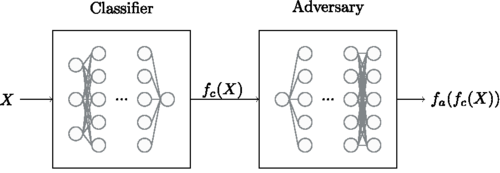
\includegraphics[width=\textwidth]{images/annarchitecture.jpeg}
    \caption{Caption}
    \label{fig:achitecture}
\end{figure}


The input data originate from the substructure algorithms implemented in FastJet, based on simulated data. Thus, it is already known whether those data have substructure or what type it is.


\section{Aspects of the network}

\subsection{The classifier}
The classifier neural network has eleven input variables, three fully connected hidden layers each with 300 nodes, and a single output node. Its inputs are jet substructure variables, similar to jettiness and D2 that were discussed in subsection \ref{ch:sub_alg}.

\subsection{The adversarial}
The adversarial network has a single input node, 50 nodes and an output layer corresponding to the guessed properties of the jet in question.

\subsection{Input data}
The current input file used for training the network, consists of 22 million jets. Each jet takes up 96 bytes of memory, thus the input data file take up around 2GB of memory.

The data set used for experiments is divided into two parts. 80\% of the data are used for training, while the other 10\% for testing. 

\subsection{Training stages}
The training of the jet substructure neural network has three stages. 

Initially the classifier is trained for a number of epochs; typically 200. Then, the adversary is trained for 10 epochs while the classifier is fixed. Finally, the combination of the classifier and the adversary are trained together for another 200 epochs.


\section{Technical characteristics}
Under the hood, the jet substructure adversarial neural network is written in Python and is composed of around 700 thousand lines of code. It makes use of Keras on top of Tensor-flow. 

\subsection{Tensor-flow}
TensorFlow is an open-source framework created by Google for creating Deep Learning models. It allows for instant creation of trained production models and is currently the number one deep learning framework.

No focus will be given on tensor-flow, in this project, as it just serves as the base for Keras.

\subsection{Keras}

Keras \cite{keras} is a high-level neural networks API, able to run on top of TensorFlow. Usually, application writtein using Keras cannot match the speed of neural networks written natively in tensor-flow; the strong weapon of Keras is the simplicity of creating neural networks. In a few lines of code a full working network can be implemented. It is able to run on both CPU and GPU.

\subsubsection{Keras sample code}
\lstinputlisting[language=python, caption=fix me please. Taken from \cite{keras2}.,escapechar=|]{codes/keras.py}

\subsubsection{Batch size}
A Keras parameter that will become important in the next chapter is the batch size. The batch size states the amount of input data that the network should be trained on before the weights are evaluated again. Choosing the optimal batch size value is not an easy task.

In case the batch size is too small, the calculated values have less statistical significance and the weights might jump around. As a result, the neural network converges slower but this way it may be easier to escape any local minimum.

For very big batch size, the network converges much faster but the weights can be stack in local minima and reduce the generalisation ability of the model. For more information, read \cite{keskar2016large}.

In case the neural network is trained on a GPU, the batch size also controls one more technical aspect: the amount of data that will be copied at once to the GPU card. If the batch size is small less data are being copied, which is faster but doesn't keep the kernels busy for much time. For big batch sizes, the kernels have more work to do, per batch delivered, but maybe the whole batch doesn't fit in the GPU card's memory.  


\section{Installation}\label{nninstall}
        The software currently resides in a git repository\cite{anngit} and the project's wiki includes a quick start section. The installation instructions are simple. Clone the git repository and run an installation bash shell script.
        
        Under the hood, the install script, initially installs anaconda, a sandboxed environment for scientific python. In a similar way to the singularity container (discussed on section \ref{ch:singularity}), anaconda provides the ability to create environments that encapsulate a collection of software. 
        
        After the installation of anaconda, the script creates two anaconda environments, for CPU and GPU usage. In each of those environments, a number of software is being installed. The most important of those are Python, Tensor-flow, Keras and CERN Root. The last is a scientific software framework heavily utilised at CERN. The difference between the two environments is that the GPU environment installs a variation of Tensorflow with GPU support. 
    


\section{Usage}\label{nnuse}
        With the software installed, in order to enter the appropriate anaconda environment and load the necessary modules, the user can execute a script
    \begin{lstlisting}
            source activate.sh <<argument>>\end{lstlisting}
        where the argument can either be \textbf{cpu} or \textbf{gpu}, depending whether the user desires GPU support or not. The loaded modules depend on the system.

        A shell script is provided with the source code, that when ran downloads the input file for the software. Afterwards, to execute the software, the following command should be issued
        
        \begin{lstlisting}
python -m run.adversarial.train  <<list of optional arguments>>\end{lstlisting}
        where the arguments (those that will be used during this work) are
        \begin{itemize}
            \item \textbf{--train}\verb|           |Train both the classifier and adversary
            \item \textbf{--train-classifier}\verb|    |Train only the classifier
            \item \textbf{--train-adversarial}\verb|  |Train only the adversary
            \item \textbf{--cpu}\verb|            |Run on CPU (default)
            \item \textbf{--gpu}\verb|            |Run on GPU
            \item \textbf{--devices DEVICES}\verb|  |Number of GPU devices to use (default value is 1)
            \item \textbf{--config CONFIG}\verb|   |The path to the configuration file
            \item \textbf{--help}\verb|            |Show a help message and exit
            \item \textbf{--tensorboard}\verb|      |Use TensorBoard, a visualisation tool for TensorFlow



        \end{itemize}
     
        Note that the training strategy depends in the existence of training results. If the neural network has been trained already, the default strategy is to not train unless forced by an argument.
        
        Appendix \ref{ch:nnoutput} shows the output of the neural network when ran with the \verb|--|train flag. 